%%%%%%%%%%%%%%%%%%%%%%%%%%%%%%%%%%%%%%%%%
% Document Author: Plinio H. Vargas
% Course: CS-532, Spring 2016 at Old Dominion University
%
% Structured General Purpose Assignment
% LaTeX Template
%
% This template has been downloaded from:
% http://www.latextemplates.com
%
% Original template author:
% Ted Pavlic (http://www.tedpavlic.com)
%
% Note:
% The \lipsum[#] commands throughout this template generate dummy text
% to fill the template out. These commands should all be removed when 
% writing assignment content.
%
%%%%%%%%%%%%%%%%%%%%%%%%%%%%%%%%%%%%%%%%%
%----------------------------------------------------------------------------------------
%	PACKAGES AND OTHER DOCUMENT CONFIGURATIONS
%----------------------------------------------------------------------------------------

\documentclass{article}

\usepackage{fancyhdr} % Required for custom headers
\usepackage{lastpage} % Required to determine the last page for the footer
\usepackage{extramarks} % Required for headers and footers
\usepackage{listings}
\usepackage{graphicx} % Required to insert images
\usepackage{lipsum} % Used for inserting dummy 'Lorem ipsum' text into the template
\usepackage[bookmarks,bookmarksopen,bookmarksdepth=2]{hyperref} % for bookmarks
\usepackage{enumerate}
\usepackage{csquotes} % for quoting things
\usepackage{multirow}
\usepackage{amsmath}
\usepackage{caption}
\usepackage{navigator}%\usepackage{caption}
\usepackage[shortlabels]{enumitem}
\usepackage{enumitem}
\usepackage{lmodern}
\usepackage[utf8]{inputenc}
%\usepackage[table]{xcolor}% http://ctan.org/pkg/xcolo
\usepackage[dvipsnames]{xcolor}
\usepackage{longtable}
\usepackage{textcomp}
\usepackage{url}
\usepackage{import}
\usepackage{float}
\usepackage{dashrule} % for dashline
\usepackage{keystroke}
\usepackage{amssymb}

\lstdefinestyle{numbers}
{ frame=tb,
  language=python,
  aboveskip=3mm,
  belowskip=3mm,
  showstringspaces=false,
  columns=flexible,
  basicstyle={\small\ttfamily},
  numbers=left,
  numberstyle=\tiny\color{gray},
  keywordstyle=\color{blue},
  commentstyle=\color{OliveGreen},
  stringstyle=\color{purple},
  breaklines=true,
  breakatwhitespace=true,
  tabsize=3
}

\lstdefinestyle{nonumbers}
{ frame=shadowbox,
  language=python,
  aboveskip=3mm,
  belowskip=3mm,
  showstringspaces=false,
  columns=flexible,
  basicstyle={\small\ttfamily},
  numbers=none,
  numberstyle=\tiny\color{gray},
  keywordstyle=\color{blue},
  commentstyle=\color{OliveGreen},
  stringstyle=\color{purple},
  breaklines=true,
  breakatwhitespace=true,
  tabsize=3
}

\lstdefinestyle{mybox}
{
	basicstyle={\small\ttfamily},
    numbers=left,
    numberstyle=\tiny\color{gray},
    stepnumber=1,
    numbersep=5pt,
    showspaces=false, % don't show spaces by adding underscores
    showstringspaces=false, % don't underline spaces in strings
    showtabs=false, % don't show tabs with underscores
    frame=shadowbox,
    tabsize=4,
    captionpos=b,
    breaklines=true,
    breakatwhitespace=false,
  	keywordstyle=\color{blue},
	commentstyle=\color{OliveGreen},
  	stringstyle=\color{purple},    
    rulesepcolor=\color{red!20!green!20!blue!20},
    numberbychapter=false,
    stringstyle=\color{purple},
}


\providecommand{\providehyphenmins}[2]{}

% Margins
\topmargin=-0.45in
\evensidemargin=0in
\oddsidemargin=0in
\textwidth=6.5in
\textheight=9.0in
\headsep=0.25in 

\linespread{1.1} % Line spacing
\newcommand*{\medtau}{\mathbin{\scalebox{1.5}{$\tau$}}}% increase size of tau
\newcommand*{\medtaub}{\mathbin{\scalebox{1.5}{$\tau_b$}}}% increase size of tau_b
\newcommand\multibrace[3]{\rdelim\}{#1}{3mm}[\pbox{#2}{#3}]}

% Set up the header and footer
\pagestyle{fancy}
\lhead{\hmwkAuthorName} % Top left header
\chead{\hmwkShortClass\ (\hmwkClassInstructor\ \hmwkClassTime): \hmwkShortTitle} % Top center header
%\rhead{\firstxmark} % Top right header
\rhead{} % Top right header
\lfoot{\lastxmark} % Bottom left footer
\cfoot{} % Bottom center footer
\rfoot{Page\ \thepage\ of\ \pageref{LastPage}} % Bottom right footer
\renewcommand\headrulewidth{0.4pt} % Size of the header rule
\renewcommand\footrulewidth{0.4pt} % Size of the footer rule

\setlength\parindent{0pt} % Removes all indentation from paragraphs

%----------------------------------------------------------------------------------------
%	DOCUMENT STRUCTURE COMMANDS
%	Skip this unless you know what you're doing
%----------------------------------------------------------------------------------------

% Header and footer for when a page split occurs within a problem environment
\newcommand{\enterProblemHeader}[1]{
\nobreak\extramarks{#1}{#1 continued on next page\ldots}\nobreak
\nobreak\extramarks{#1 (continued)}{#1 continued on next page\ldots}\nobreak
}

% Header and footer for when a page split occurs between problem environments
\newcommand{\exitProblemHeader}[1]{
\nobreak\extramarks{#1 (continued)}{#1 continued on next page\ldots}\nobreak
\nobreak\extramarks{#1}{}\nobreak
}

\newcounter{sub}[section]
\newenvironment{sub}[1][]{\stepcounter{sub}\thesub #1}{ }

\setcounter{secnumdepth}{0} % Removes default section numbers
\newcounter{homeworkProblemCounter} % Creates a counter to keep track of the number of problems
\newcommand{\sectionNumber}{\arabic{homeworkProblemCounter}.\sub }


\newcommand{\homeworkProblemName}{}
\newenvironment{homeworkProblem}[1][Problem \arabic{homeworkProblemCounter}]{ % Makes a new environment called homeworkProblem which takes 1 argument (custom name) but the default is "Problem #"
\stepcounter{homeworkProblemCounter} % Increase counter for number of problems
\setcounter{sub}{0}
\renewcommand{\homeworkProblemName}{#1} % Assign \homeworkProblemName the name of the problem
\
\section{\homeworkProblemName} % Make a section in the document with the custom problem count
\enterProblemHeader{\homeworkProblemName} % Header and footer within the environment
}{
\exitProblemHeader{\homeworkProblemName} % Header and footer after the environment
}

\newcommand{\problemAnswer}[1]{ % Defines the problem answer command with the content as the only argument
\noindent\framebox[\columnwidth][c]{\begin{minipage}{0.98\columnwidth}#1\end{minipage}} % Makes the box around the problem answer and puts the content inside
}

\newcommand{\homeworkSectionName}{}
\newenvironment{homeworkSection}[1]{ % New environment for sections within homework problems, takes 1 argument - the name of the section
\renewcommand{\homeworkSectionName}{#1} % Assign \homeworkSectionName to the name of the section from the environment argument
\subsection{\homeworkSectionName} % Make a subsection with the custom name of the subsection
\enterProblemHeader{\homeworkProblemName\ [\homeworkSectionName]} % Header and footer within the environment
}{
\enterProblemHeader{\homeworkProblemName} % Header and footer after the environment
}
   
%----------------------------------------------------------------------------------------
%	NAME AND CLASS SECTION
%----------------------------------------------------------------------------------------

\newcommand{\hmwkTitle}{\\Assignment\ \#7: \\User-Collected Data} % Assignment title
\newcommand{\hmwkShortTitle}{Assignment 7} % Assignment title
\newcommand{\hmwkDueDate}{Thursday,\ March 31,\ 2016} % Due date
\newcommand{\hmwkClass}{CS-432/532 Introduction to Web Science} % Course/class
\newcommand{\hmwkShortClass}{CS-432/532 Web Science} % Course/class
\newcommand{\hmwkClassTime}{- Spring 2016} % Class/lecture time
\newcommand{\hmwkClassInstructor}{Dr.  Michael L. Nelson} % Teacher/lecturer
\newcommand{\hmwkAuthorName}{Plinio Vargas} % Your name
\newcommand{\hmwkAuthorEmail}{pvargas@cs.odu.edu} % Your name
%------------------------------------------------------------
% Algorithm declaration
%------------------------------------------------------------
\lstnewenvironment{algorithm}[1][] %defines the algorithm listing environment
{   
    %\refstepcounter{nalg} %increments algorithm number
    \captionsetup{labelsep=colon} %defines the caption setup for: it ises label format as the declared caption label above and makes label and caption text to be separated by a ':'
    \lstset{ %this is the stype
        frame=tB,
        numbers=left, 
        mathescape=true,
        numberstyle=\tiny,
        basicstyle={\small\ttfamily}, 
        keywordstyle=\color{blue}\bfseries\em,
        keywords={,input, output, return, 
                   datatype, function, in, 
                   if, else, for, foreach, 
                   while, write, begin, end, 
        } %add the keywords you want, or load a language as Rubens explains in his comment above.
        numbers=left,
        xleftmargin=.04\textwidth,
        #1 % this is to add specific settings to an usage of this environment (for instnce, the caption and referable label)
    }
}
{}
%----------------------------------------------------------------------------------------
%	TITLE PAGE
%----------------------------------------------------------------------------------------

\title{
\vspace{2in}
\textmd{\textbf{\hmwkClass:\ \hmwkTitle}}\\
\normalsize\vspace{0.1in}\small{Due\ on\ \hmwkDueDate}\\
\vspace{0.1in}\large{\textit{\hmwkClassInstructor\ }}
\vspace{3in}
}

\author{\textbf{\hmwkAuthorName} \\ \hmwkAuthorEmail}
\date{} % Insert date here if you want it to appear below your name

%----------------------------------------------------------------------------------------
%	EMBEDDED FILE
%----------------------------------------------------------------------------------------
%\embeddedfile{KarateClub}{../KarateClub.py}
%\embeddedfile{DrawOriginalClub}{../DrawOriginalClub.py}
%----------------------------------------------------------------------------------------
%	START OF DOCUMENT
%----------------------------------------------------------------------------------------
\begin{document}

\clearpage\maketitle
\thispagestyle{empty}

%----------------------------------------------------------------------------------------
%	TABLE OF CONTENTS
%----------------------------------------------------------------------------------------

%\setcounter{tocdepth}{1} % Uncomment this line if you don't want subsections listed in the ToC

\newpage
\clearpage\tableofcontents
\listoffigures
\lstlistoflistings
\listoftables

\thispagestyle{empty}
\newpage
\setcounter{page}{1}

The goal of this project is to use the basic recommendation principles we have learned for user-collected data. You will modify the code given to you which performs movie recommendations from the MovieLense data sets.\\

The MovieLense data sets were collected by the GroupLens Research Project at the University of Minnesota during the seven-month period from September 19th, 1997 through April 22nd, 1998.  We are using the  \enquote{100k dataset}; available for download from: \url{http://grouplens.org/datasets/movielens/100k/}\\

There are three files which we will use:
\begin{enumerate}[1. ]

\item  u.data: 100,000 ratings by 943 users on 1,682 movies. Each  user has rated at least 20 movies. Users and items are numbered consecutively from 1. The data is randomly ordered. This is a tab separated list of:\\

user id | item id | rating | timestamp\\

The time stamps are unix seconds since 1/1/1970 UTC.\\

Example:\\

\begin{tabular}{l l l l}
196  &   242  &   3   &    881250949\\
186  &   302  &   3   &    891717742\\
22   &   377  &   1   &    878887116\\
244  &   51   &   2   &    880606923\\
166  &   346  &   1   &    886397596\\
298  &   474  &   4   &    884182806\\
115  &   265  &   2   &    881171488\\
\end{tabular}

\item  u.item: Information about the 1,682 movies. This is a tab separated list of\\

movie id \texttt{|} movie title \texttt{|} release date \texttt{|} video release date \texttt{|} IMDb URL \texttt{|} unknown \texttt{|} Action \texttt{|} Adventure \texttt{|} Animation \texttt{|}Children's \texttt{|} Comedy \texttt{|} Crime \texttt{|} Documentary \texttt{|} Drama \texttt{|} Fantasy \texttt{|} Film-Noir \texttt{|} Horror \texttt{|} Musical \texttt{|} Mystery \texttt{|} Romance \texttt{|} Sci-Fi \texttt{|} Thriller \texttt{|} War \texttt{|} Western \texttt{|}\\

The last 19 fields are the genres, a 1 indicates the movie is of that genre, a 0 indicates it is not; movies can be in several genres at once. The movie ids are the ones used in the u.data data set.\\

Example:\\

\scriptsize
\hspace*{-23mm}161\texttt{|}Top Gun (1986)\texttt{|}01-Jan-1986\texttt{|}\texttt{|}http://us.imdb.com/M/title-exact?Top\%20Gun\%20(1986)\texttt{|}0\texttt{|}1\texttt{|}0\texttt{|}0\texttt{|}0\texttt{|}0\texttt{|}0\texttt{|}0\texttt{|}0\texttt{|}0\texttt{|}0\texttt{|}0\texttt{|}0\texttt{|}0\texttt{|}1\texttt{|}0\texttt{|}0\texttt{|}0\texttt{|}0\\
\hspace*{-23mm}162\texttt{|}On Golden Pond (1981)\texttt{|}01-Jan-1981\texttt{|}\texttt{|}http://us.imdb.com/M/title-exact?On\%20Golden\%20Pond\%20(1981)\texttt{|}0\texttt{|}0\texttt{|}0\texttt{|}0\texttt{|}0\texttt{|}0\texttt{|}0\texttt{|}0\texttt{|}1\texttt{|}0\texttt{|}0\texttt{|}0\texttt{|}0\texttt{|}0\texttt{|}0\texttt{|}0\texttt{|}0\texttt{|}0\texttt{|}0 \\
\hspace*{-23mm}163\texttt{|}Return of the Pink Panther, The (1974)\texttt{|}01-Jan-1974\texttt{|}\texttt{|}http://us.imdb.com/M/title-exact?Return\%20of\%20the\%20Pink\%20Panther,\%20The\\

\normalsize
\item  u.user: Demographic information about the users. This is a tab
separated list of:\\

user id \texttt{|} age \texttt{|} gender \texttt{|} occupation \texttt{|} zip code\\

The user ids are the ones used in the u.data data set.\\

Example:\\

1\texttt{|}24\texttt{|}M\texttt{|}technician\texttt{|}85711 \\
2\texttt{|}53\texttt{|}F\texttt{|}other\texttt{|}94043 \\
3\texttt{|}23\texttt{|}M\texttt{|}writer\texttt{|}32067 \\
4\texttt{|}24\texttt{|}M\texttt{|}technician\texttt{|}43537 \\
5\texttt{|}33\texttt{|}F\texttt{|}other\texttt{|}15213 \\

The code for reading from the u.data and u.item files and creating recommendations is described in the book Programming Collective Intelligence.  Feel free to modify the PCI code to answer the following questions.
\end{enumerate}
%----------------------------------------------------------------------------------------
%	Problem 1
%----------------------------------------------------------------------------------------
\begin{homeworkProblem}% Custom section title
\vspace*{10pt} % Question
 Find 3 users who are closest to you in terms of age, gender, and occupation.  For each of those 3 users:
\begin{itemize}
\item what are their top 3 favorite films?
\item bottom 3 least favorite films?
\end{itemize}

Based on the movie values in those 6 tables (3 users X (favorite + least)), choose a user that you feel is most like you.  Feel free to note any outliers (e.g., \enquote{I mostly identify with user 123, except I did not like 'Ghost' at ll}).\\  

This user is the \enquote{substitute you}. \\

\subsection{1.1 Approach}
There were three approaches considered in order to answer the questions in this assignment:
\begin{enumerate}[a. ]
	\item Using R to upload, query and analyze the data.
	\item Saving data as string, manipulating the data using python scripts.
	\item Following \cite{ci} advice and storing data into a database for manipulation.
\end{enumerate}
We followed the latest approach. PostgreSQL was selected as our DBMS. Various bash shells and python scripts were created to upload and manipulate the data from PostgreSQL. Very small modifications were made to the solutions available in \cite{ci} in order to be adapted into Python 3.4 syntax.\\

First, we created the database \textbf{cs752\_db} using bash shell \textit{CreateDb.sh}:

\lstinputlisting[language=bash,
                 style=mybox, 
                 captionpos=t,
                 caption={CreateDb.sh},
                 label={lst:createdb},
				 linerange={1-14},
				 firstnumber=1              
                 ]
{../CreateDb.sh}
The script created the database and some extensions.\\

Second, we created the tables and populated them using a bash shell and python. The section below is just a portion of the script showing the syntax of creating user's table \textit{user\_tb} from the command line:
\lstinputlisting[language=bash,
                 style=mybox, 
                 captionpos=t,
                 caption={Creating Table Using CreatePopulateTbls.sh},
                 label={lst:create-tbl},
				 linerange={21-30},
				 firstnumber=21              
                 ]
{../CreatePopulateTbls.sh}
Below is another portion of the same script, but showing how the table gets populated:

\lstinputlisting[language=bash,
                 style=mybox, 
                 captionpos=t,
                 caption={Loading Table Via CreatePopulateTbls.sh Script},
                 label={lst:populate-tbl},
				 linerange={61-70},
				 firstnumber=61              
                 ]
{../CreatePopulateTbls.sh}
\vspace{5mm}
The data set obtained from \url{http://grouplens.org/datasets/movielens/100k/} was uploaded into the corresponding \textbf{postgres} tables shown below:

\begin{center}
u.data $\to$ rating\_tb\\
u.item $\to$ movie\_tb\\
t.user $\to$ user\_tbl\\
\end{center}

Once the tables were created (line 1-30), the remaining portion of the script populates the data into the respective tables by using \enquote{COPY} instruction. This instruction is a display of the text files via \textit{python}, which after given the data-fields character separators replace them with a tab for \textbf{postgres}. For example:\\
\lstinputlisting[language=python,
                 style=mybox, 
                 captionpos=t,
                 caption={Example of Simple Data Upload: TransferUserData.py},
                 label={lst:user},
				 linerange={7-12},
				 firstnumber=7              
                 ]
{../TransferUserData.py}
Listing \ref{lst:user} is the simplest form of data upload. In other cases is a little more complex because we have to account for missing data fields or a misalignment for character separators in the data. This cannot be done in advance; it is done based on trial and error, patching the mistakes as the data gets uploaded into the tables.
\lstinputlisting[language=python,
                 style=mybox, 
                 captionpos=t,
                 caption={Example of Complex Data Upload: TransferMoviesData.py},
                 label={lst:movies},
				 linerange={11-29},
				 firstnumber=11              
                 ]
{../TransferMoviesData.py}

The example in Listing \ref{lst:movies} is more complex than Listing \ref{lst:user}. Listing \ref{lst:movies} accounts for a non-uniform data. During data upload there was a movie titled \textit{unknown} without a date field, so instead of discarding this record a data field was added (lines 16-17). In addition, the script is compressing 19 genres data-fields into a single data-field (lines 22-23).

\newpage
\subsection{1.2 Solution}
\subsubsection{1.2.1 3-Users Closest to Me in Terms of Age, Gender, and Occupation}
To find 3 users who are closest to me in terms of age, gender, and occupation, we performed a search for all male students between the ages of 35 to 45 years old limiting to 3 tuples. That search yielded the following results:\\

\begin{lstlisting}[style=nonumbers, keywords={select, from, where, limit, and}]
		select * from user_tb 
		where age >= 35 and age <= 45 and
		occupation = 'student' and gender = 'M'
		limit 3;
\end{lstlisting}

%----------------------------------------------------------------------------------------
%	Table1
%----------------------------------------------------------------------------------------
\import{./}{table-1.tex}

\newpage
\subsubsection{1.2.2 3-Users Closest to Me Top 3 Favorite Films}
To answer this question 3 queries were performed in \textbf{postgres}:\\
\begin{figure}[hr]
\center
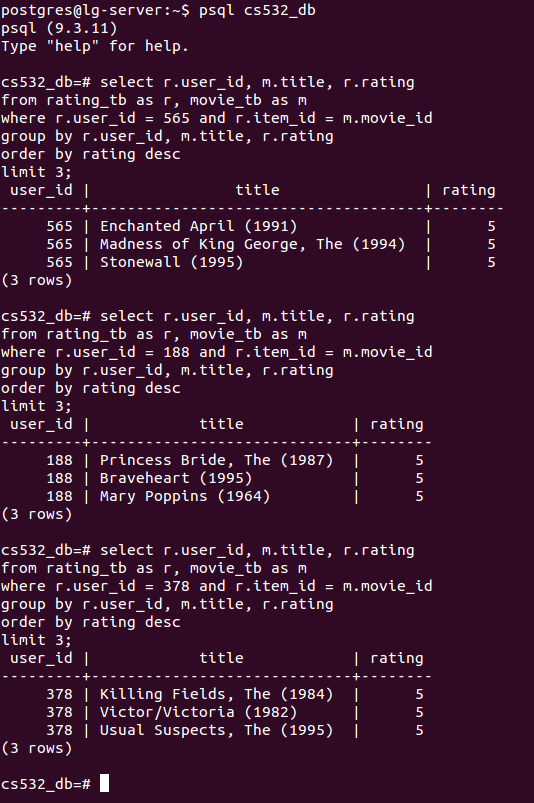
\includegraphics[scale=0.5]{images/mostfavorite.png}
\end{figure}

\vspace{5mm}
The query combined \textit{rating\_tb} with \textit{movie\_tb} sorted by the ranking field in a decedent fashion, limiting to only 3 tuples, and then extracting only the desired fields: \textbf{user\_id}, movie \textbf{title} and \textbf{rating}.\\

Then, to obtain the highest ranking movies from user \textcolor{blue}{188} we query:
\begin{lstlisting}[style=nonumbers, keywords={select, from, where, limit, and, group, as, order, by}]
	select r.user_id, m.title, r.rating
	from rating_tb as r, movie_tb as m
	where r.user_id = 188 and r.item_id = m.movie_id
	group by r.user_id, m.title, r.rating
	order by rating desc
	limit 3;
\end{lstlisting}
Yielding table:


%----------------------------------------------------------------------------------------
%	Table Highest ranking for 188
%----------------------------------------------------------------------------------------
\import{./}{table-2.tex}

\vspace{10mm}
Then, to obtain the 3-highest movies ranked by user 378 we just changed the user\_id field to 378, leaving everything else the same:
\begin{lstlisting}[style=nonumbers, keywords={select, from, where, limit, and, group, as, order, by}]
	select r.user_id, m.title, r.rating
	from rating_tb as r, movie_tb as m
	where r.user_id = 378 and r.item_id = m.movie_id
	group by r.user_id, m.title, r.rating
	order by rating desc
	limit 3;
\end{lstlisting}

Yielding table:
%----------------------------------------------------------------------------------------
%	Table Highest ranking for user 378
%----------------------------------------------------------------------------------------
\import{./}{table-3.tex}


The same applies to user 565:
\begin{lstlisting}[style=nonumbers, keywords={select, from, where, limit, and, group, as, order, by}]
	select r.user_id, m.title, r.rating
	from rating_tb as r, movie_tb as m
	where r.user_id = 565 and r.item_id = m.movie_id
	group by r.user_id, m.title, r.rating
	order by rating desc
	limit 3;
\end{lstlisting}

Yielding table:
%----------------------------------------------------------------------------------------
%	Table Highest ranking for user 565
%----------------------------------------------------------------------------------------
\import{./}{table-4.tex}

\subsubsection{1.2.3 3-Users Closest to Me Least 3 Favorite Films}
Different from sub-section before, in order to obtain the least favorite ranked films from selected users the only change in our query is to order the ranking field from descending fashion in an ascending one. Then, to get the least favorite ranked movies by user \textcolor{blue}{188} we can query \textbf{postgres} \textit{cs752\_db}:

\begin{lstlisting}[style=nonumbers, keywords={select, from, where, limit, and, group, as, order, by}]
	select r.user_id, m.title, r.rating
	from rating_tb as r, movie_tb as m
	where r.user_id = 188 and r.item_id = m.movie_id
	group by r.user_id, m.title, r.rating
	order by rating asc
	limit 3;
\end{lstlisting}

Yielding table:
%----------------------------------------------------------------------------------------
%	Table lowest ranking for user 188
%----------------------------------------------------------------------------------------
\import{./}{table-5.tex}

For user 378:

\begin{lstlisting}[style=nonumbers, keywords={select, from, where, limit, and, group, as, order, by}]
	select r.user_id, m.title, r.rating
	from rating_tb as r, movie_tb as m
	where r.user_id = 378 and r.item_id = m.movie_id
	group by r.user_id, m.title, r.rating
	order by rating asc
	limit 3;
\end{lstlisting}

Yielding table:
%----------------------------------------------------------------------------------------
%	Table lowest ranking for user 378
%----------------------------------------------------------------------------------------
\import{./}{table-6.tex}

Finally, for user 565 we may query:

\begin{lstlisting}[style=nonumbers, keywords={select, from, where, limit, and, group, as, order, by}]
	select r.user_id, m.title, r.rating
	from rating_tb as r, movie_tb as m
	where r.user_id = 565 and r.item_id = m.movie_id
	group by r.user_id, m.title, r.rating
	order by rating asc
	limit 3;
\end{lstlisting}

Yielding table:
%----------------------------------------------------------------------------------------
%	Table lowest ranking for user 565
%----------------------------------------------------------------------------------------
\import{./}{table-7.tex}

\subsubsection{1.2.4 Substitute Me}\label{sec:1.2.4}
Selecting substitute me was a painful (\textbf{water-boarding}) decision. I could not identify with user \textcolor{blue}{188}, although I would rank \enquote{Braveheart (1995)} equally with a 5, \enquote{Princess Bride, The (1987)} and \enquote{Mary Poppins (1964)} would be around 2 instead of 5.\\

I am very distant from user \textcolor{blue}{565}, all the highest ranked films by \textcolor{blue}{565} would be in my lowest ranked film selections. \\

I am not that close with user \textcolor{blue}{378} either, his highest ranked films I would given them a 3 rate selection.\\

Solution:
\begin{lstlisting}[style=nonumbers, keywords={378}]
	User 378 was selected as substitute me.
\end{lstlisting}
\end{homeworkProblem}


%----------------------------------------------------------------------------------------
%	Problem 2 
%----------------------------------------------------------------------------------------
\newpage
\begin{homeworkProblem}
Which 5 users are most correlated to the substitute you? Which 5 users are least correlated (i.e., negative correlation)?

\subsection{2.1 Approach}
To answer questions 2 through 4, a Python program was created (\textit{GetCorr.py}). Its output is displayed below:

\begin{lstlisting}[style=nonumbers]
/usr/bin/python3.4 "/DiskStation/CS-532 Webscience/a7/GetCorr.py"
Starting Time: Wed,  Mar 30, 2016 at 17:33:16

Top 5 most correlated substitute me
+----------+----------------+
| Movie_id | Recomm Ranking |
+----------+----------------+
|   369    |     1.000      |
|   651    |     0.878      |
|   841    |     0.866      |
|   341    |     0.866      |
|   149    |     0.818      |
+----------+----------------+


Bottom 5 correlated substitute me
+----------+----------------+
| Movie_id | Recomm Ranking |
+----------+----------------+
|   866    |     -0.730     |
|   677    |     -0.681     |
|   723    |     -0.614     |
|   812    |     -0.603     |
|   471    |     -0.600     |
+----------+----------------+


             Substitute me 5 top unseen movie recommendations

+----------+---------------------------------------------------+----------------+
| Movie_id |                Title                              | Recomm Ranking |
+----------+---------------------------------------------------+----------------+
|   1189   | Prefontaine (1997)                                |     5.000      |
|   1653   | Entertaining Angels: The Dorothy Day Story (1996) |     5.000      |
|   1617   | Hugo Pool (1997)                                  |     5.000      |
|   1599   | Someone Else's America (1995)                     |     5.000      |
|   1536   | Aiqing wansui (1994)                              |     5.000      |
+----------+---------------------------------------------------+----------------+



            Substitute me 5 least unseen movie recommendations

+----------+---------------------------------------------------+----------------+
| Movie_id |                Title                              | Recomm Ranking |
+----------+---------------------------------------------------+----------------+
|   314    | 3 Ninjas: High Noon At Mega Mountain (1998)       |     1.000      |
|   437    | Amityville 1992: It's About Time (1992)           |     1.000      |
|   439    | Amityville: A New Generation (1993)               |     1.000      |
|   599    | Police Story 4: Project S (Chao ji ji hua) (1993) |     1.000      |
|   784    | Beyond Bedlam (1993)                              |     1.000      |
+----------+---------------------------------------------------+----------------+

End Time:  Wed,  Mar 30, 2016 at 17:33:17
Execution Time: 0.72 seconds

Process finished with exit code 0
\end{lstlisting}

\vspace{5mm}
We used \textit{pysycopg2} python library to connect with the database and the \textit{sim\_pearson} function developed in \cite{ci}. The function expects the user preferences. \textbf{GetCorr.py} stores substitute me preferences in variable substitute\_me (lines 33-36).

\lstinputlisting[language=python,
                 style=mybox, 
                 captionpos=t,
                 caption={Finding Closest Substitute Me Match: GetCorr.py},
                 label={lst:get-corr},
				 linerange={33-52},
				 firstnumber=33              
                 ]
{../GetCorr.py}

\vspace{5mm}
\textbf{Substitute me} preference information is entered into an iteration that compares with everyone else's preference (lines 40 - 52). The correlation is calculated by passing \textbf{substitute me} preference with the other user preference to function \textit{sim\_pearson}. The result of each calculation is stored in a table \textit{corr\_table} in line 52.

If we sort \textit{corr\_table} in ascending order by ranking, the bottom portion will correspond to the closest correlation to \textbf{substitute me} in terms of moving ranking criteria. The top portion of the table will be the opposite.
\subsection{2.2 Solution}
\subsubsection{2.2.1 5-Users Most Correlated to the Substitute Me}
%----------------------------------------------------------------------------------------
%	Table Top 5 Correlated Subustitute Me
%----------------------------------------------------------------------------------------
\import{./}{table-8.tex}

\subsubsection{2.2.1 5-Users Least Correlated to the Substitute Me}
%----------------------------------------------------------------------------------------
%	Table 5-Users Least Correlated to the Substitute Me
%----------------------------------------------------------------------------------------
\import{./}{table-9.tex}

\end{homeworkProblem}

%----------------------------------------------------------------------------------------
%	Problem 3
%----------------------------------------------------------------------------------------
\newpage
\begin{homeworkProblem}
Compute rankings for all the films that the substitute you hasn't seen.  Provide a list of the top 5 recommendations for films that the substitute you should see.  Provide a list of the bottom 5 recommendations (i.e., films the substitute you is almost certain to hate).?

\subsection{3.1 Approach}
The preference of all users was stored in variable \textit{all\_prefs} (line 46 in Listin \ref{lst:get-corr}). This information along with my user\_id is passed to function \textit{getRecommendations} obtained from \cite{ci}. The result is stored in variable \textit{recommendations} which will contain the ranking of movies not yet seen by \textbf{substitute me} ordered from least likely desired recommended preference to the most likely recommended preference.

Then, to answer the question, we take the top or bottom portion of the array.

\subsection{3.2 Solution}
\subsubsection{3.2.1 Top 5 Recommendations of Unseen films for Substitute Me }
%----------------------------------------------------------------------------------------
%	Table Top 5 Substitute Me Recommendations of Unseen films
%----------------------------------------------------------------------------------------
\import{./}{table-10.tex}

\subsubsection{3.2.2 Bottom 5 Recommendations of Unseen films for Substitute Me}
%----------------------------------------------------------------------------------------
%	Table Top 5 Substitute Me Recommendations of Unseen films
%----------------------------------------------------------------------------------------
\import{./}{table-11.tex}

\end{homeworkProblem}

%----------------------------------------------------------------------------------------
%	Problem 4
%----------------------------------------------------------------------------------------
\newpage
\begin{homeworkProblem}
Choose your (the real you, not the substitute you) favorite and least favorite film from the data.  For each film, generate a list of the top 5 most correlated and bottom 5 least correlated films. Based on your knowledge of the resulting films, do you agree with the results?  In other words, do you personally like / dislike the resulting films?\\

\subsection{4.1 Solution}

The recommendations results are not surprising to me. As stated in \textbf{1.2.4 Substitute Me}\ref{sec:1.2.4} solution user \textcolor{blue}{378} is closest to me by default. However, the results are close in terms how I feel about \textbf{substitute me} ranking. I dislike all movies not recommended and the recommended ones I would rate them between 2 and 3, similar to the highest ranking for user \textcolor{blue}{378}.
\end{homeworkProblem}

%----------------------------------------------------------------------------------------
%	Problem 5 - Extra Credit 
%----------------------------------------------------------------------------------------
\newpage
\begin{homeworkProblem}
Rank the 1,682 movies according to the 1997/1998 MovieLense data.  Now rank the same 1,682 movies according to todays (March 2016) IMDB data (break ties based on \# of users, for example: 7.2 with 10,000 raters $>$ 7.2 with 9,000 raters).\\

Draw a graph, where each dot is a film (i.e., 1,682 dots).  The x-axis is the MovieLense ranking and the y-axis is today's IMDB ranking.\\

What is Pearon's r for the two lists (along w/ the p-value)?  Assuming the two user bases are interchangable (which might not be a good assumption), what does this say about the attitudes about the films after nearly 20 years?\\

\vspace{20mm}
\begin{center}
In progress!!
\end{center}
\end{homeworkProblem}

%----------------------------------------------------------------------------------------
%	Problem 6
%----------------------------------------------------------------------------------------
\newpage
\begin{homeworkProblem}
Repeat \#6, but IMDB data from approximately July 31, 2005.  What is the cumulative error (in days) from the desired target day of July 31, 2005?  For example, if 1 memento is from July 1, 2005 and another memento is from July 31, 2006, then the cumulative error for the two mementos is 30 days + 365 days = 385 days.\\

Note: the URIs in the MovieLens data redirect, be sure to use the final values as URI-Rs for the archives:\\

\$ curl -i -L \texttt{--}silent \enquote{http://us.imdb.com/M/title-exact?Top\%20Gun\%20(1986)}\\
HTTP/1.1 301 Moved Permanently\\
Date: Wed, 16 Mar 2016 18:37:06 GMT\\
Server: Server\\
Location: http://www.imdb.com/M/title-exact?Top\%20Gun\%20(1986)\\
Content-Length: 260\\
Content-Type: text/html; charset=iso-8859-1\\

HTTP/1.1 302 Found\\
Date: Wed, 16 Mar 2016 18:37:06 GMT\\
Server: HTTPDaemon\\
X-Frame-Options: SAMEORIGIN\\
Cache-Control: private\\
Location: http://www.imdb.com/title/tt0092099/\\
Content-Type: text/plain\\
Set-Cookie: uu=BCYuNIAbuc9FDeWcqVNAaaXLjXbagPPhyTQbhxr8CTOkHFcqkeyRbKqvk\_m6buuHjm\\HkufNf5z5S4WGfKlG6BPOhzgA-jcsRZ5Q7GW2MJP0wNI9AZMnd245Mw\_xI6spRuK\_VF2lSxUGPIRXy4d-NY-YwZkqTEZ8uTOXchLSvqBpgsDI;expires=Thu, 30 Dec 2037 00:00:00 GMT;path=/;domain=.imdb.com\\
Vary: Accept-Encoding,User-Agent\\
P3P: policyref=\enquote{http://i.imdb.com/images/p3p.xml},CP=\enquote{CAO DSP LAW CUR ADM IVAo IVDo\\ CONo OTPo OUR DELi PUBi OTRi BUS PHY ONL UNI PUR FIN COM NAV INT DEM CNT STA HEA PRE LOC GOV OTC}\\
Content-Length: 0\\

HTTP/1.1 200 OK\\
Date: Wed, 16 Mar 2016 18:37:06 GMT\\
Server: Server\\
X-Frame-Options: SAMEORIGIN\\
Content-Security-Policy: frame-ancestors 'self' imdb.com *.imdb.com *.media-imdb.com withoutabox.com *.withoutabox.com amazon.com *.amazon.com amazon.co.uk  *.amazon.co.uk amazon.de *.amazon.de translate.google.com images.google.com www.google.com www.google.co.uk search.aol.com bing.com www.bing.com\\
Content-Type: text/html;charset=UTF-8\\
Content-Language: en-US\\
Vary: Accept-Encoding,User-Agent\\
$[$deletia...$]$

\begin{center}
In progress!!
\end{center}
\end{homeworkProblem}

%----------------------------------------------------------------------------------------
%	Bibliography
%----------------------------------------------------------------------------------------
\newpage
\begin{thebibliography}{9}
%\bibitem{Lutz} 
%Lutz, Mark (2013). List and Dictionaries. \textit{Learning Python} (5th ed.). (pp. %262-263). Sebastopol, CA: O'Reilly Media.
%
\bibitem{ci}
Segarn, Toby. Programming Collective Intelligence. \textit{Building Smart Web 2.0 Application}. (pp 9). Sebastopol, CA: O'Reilly Media.

%\bibitem{zooming}
%Zooming and dragging. (n.d.) Retrieved March 10, 2016, from \url{http://bl.ocks.org/%mbostock/6123708}

\end{thebibliography}
\end{document}
